\subsubsection{Color Imaging}

Spectral information in digital sensors is typically obtained using \textit{color filter arrays} (CFAs), semi-transparent masks integrated on top of the sensor. These form a 2D periodical pattern with the three primary colors. Thus, each pixel is limited to irradiance related to the wavelength range of the respective color.

Later, the intensity values in each 2D kernel are reconstructed and interpolated, or \textit{demosaicked}, to form a single pixel with three colour channels.

The most widely used CFA configuration is Bayer RGB pattern, though many other arrangements exist~\cite{Krig2014}. Figure \ref{fig:cfabayer} shows the Bayer pattern and its exemplary position on a sensor plane.

\begin{figure}[h]
  \centering
  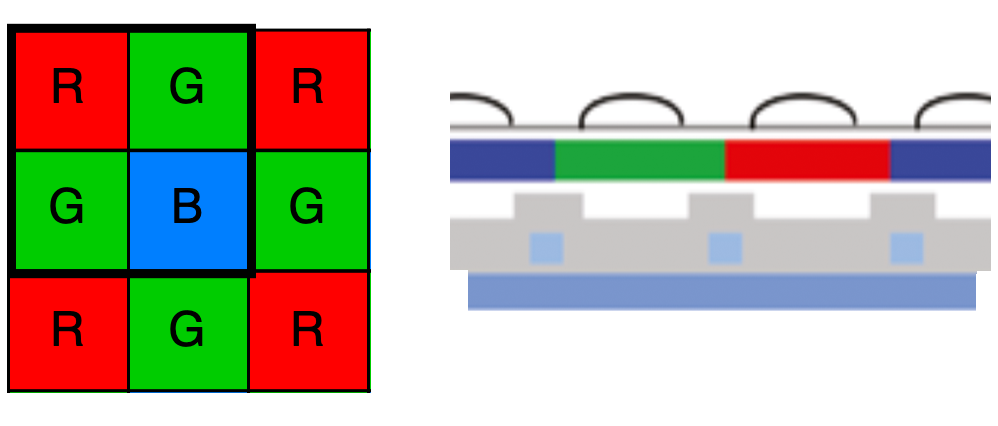
\includegraphics[width=0.8\linewidth]{imgs/cfabayer.png}
  \caption{Bayer RGB pattern and the common integrated CFA arrangement (right, via \cite{Krig2014}).}
  \label{fig:cfabayer}
  \Description{Pattern of Red, Green, Green, Blue is placed on top of the electronics.}
\end{figure}

Following problems pertain through inclusion of color information via CFA:

\begin{itemize}

\item \textbf{Aliasing}. Through demosaicking, combined spatial resolution is lowered, and under sampling rates below the Nyquist frequency, \textit{Moiré artifacts} appear.

\item \textbf{Reduced sensor sensitivity}. Part of light is blocked out and never reaches the sensor plane, and the net signal is more susceptible to noise.

\item \textbf{Crosstalk}. The optical or electrical charge in the pixels may leak towards the adjacent pixels. In CFAs, where charges depend on wavelengths and change rapidly, this results in a desaturation of the color measurements.
\end{itemize}

While these problems appear in monochromatic sensors as well, here, the errors persisting translate to false color values, which is more disturbing for the human perception \cite{Hunt2005}.

Not all effects are equally pronounced, however, attempts to alleviate one factor may result in higher impact of the others. For one, QIS sensors are unaffected by aliasing due to their small feature sizes, while conventional CMOS sensors may require designated algorithmic suppression. At the same time, smaller pixel pitches lead to severe crosstalk; even more so when the adjacent colors are different~\cite{elgendy2019color}, which is the case with the Bayer pattern. In binary sensors, the leakage means false positives, resulting in a substantially lower SNR.

\cite{Anzagira2015ColorFA} attempt to mitigate the crosstalk through the extensions of Bayer pattern. 

\begin{figure}[h]
  \centering
  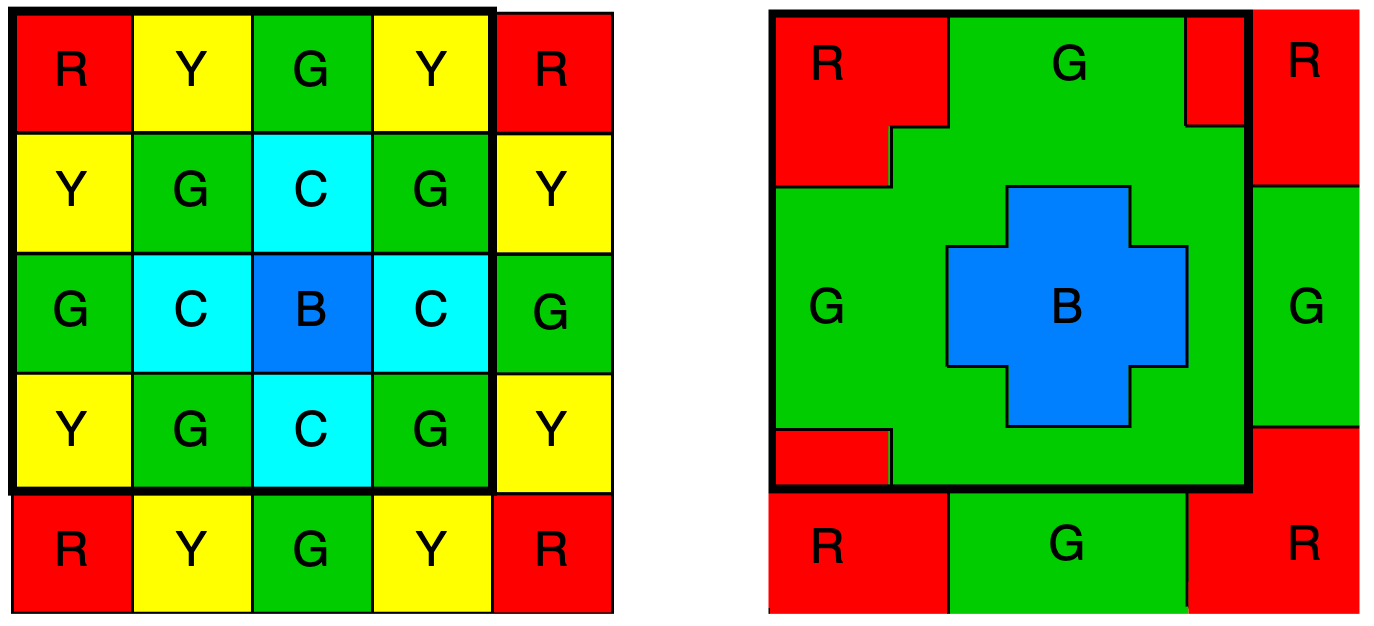
\includegraphics[width=0.7\linewidth]{imgs/cfaqis.png}
  \caption{CFA Proposals made in \cite{Anzagira2015ColorFA}.}
  \label{fig:cfaqis}
  \Description{Squared patterns for color imaging, which now include more secondary colors in the arrays or the larger bounds of the primary colors in the pattern masks.}
\end{figure}

Figure \ref{fig:cfaqis} depicts two of the proposals. On the left, the initial mosaic is expanded through secondary colors cyan, magenta, and yellow. These are positioned between the respective primary colours so that the spectral overlap is smaller. For increased light sensitivity, some of the green pixels may also be replaced with white. The second proposal expands the active color regions of the filter, leveraging the high spatial resolution of the QIS. The overlaps now occur in the regions where the pixels are halved, which can be accounted for during computations.

%Assume cross-talk to be equal for all wavelengths and only pertain in vertical and horizontal directions

\cite{elgendy2019color} focus on more than merely crosstalk mitigation, proposing design criteria for sub-diffraction limit CFAs.
Paired with a demosaicing algorithm, this should maximize spatial resolution between the channels while improving the sensitivity in general. Similarly, the demosaicking process should minimize the noise power after the light passes the filter. 

Presented in Figure \ref{fig:cfaelgendy}, the filter has a diagonal structure. The auxiliary demosaicking algorithm works on frequency selection and was found to be universally applicable, performing well in both CIS and QIS imagers.

\begin{figure}[h]
  \centering
  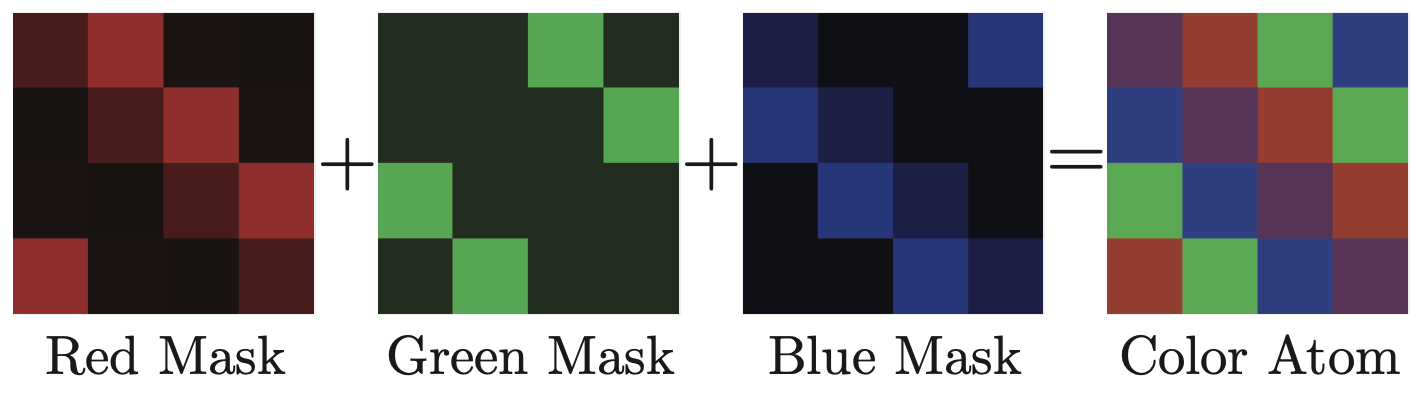
\includegraphics[width=0.7\linewidth]{imgs/cfaelgendy.png}
  \caption{CFA pattern proposed in \cite{elgendy2019color}. The patterns are positioned diagonally, with gradations, as to reduce the cross-talk between the pixels.}
  \label{fig:cfaelgendy}
  \Description{Primary colors in the pattern are positioned diagonally}
\end{figure}

In both cases, the filter kernel is larger, and the spatial resolution of the sensor is traded off for better performance in presence of crosstalk. 


 \begin{figure}[h]
  \centering
  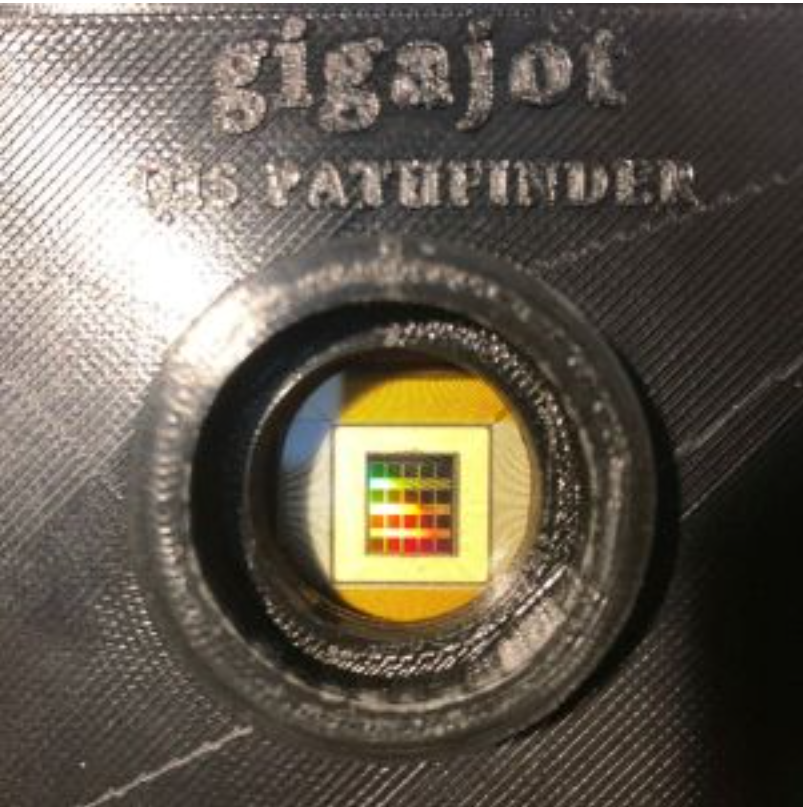
\includegraphics[width=0.5\linewidth]{imgs/qis/gigajot.png}
  \caption{Quanta imaging sensor, as seen in a Gigajot camera. Via: \cite{Gnanasambandam_2019}}
  \Description{Small industrial camera with equally small lens above it}
\end{figure}

The strictly algorithmic processing of the color image in QIS has been described and applied in \cite{Gnanasambandam_2019}, who present the QIS Pathfinder camera module developed at Gigajot Technology with a Bayer pattern color filter array implemented on-chip. 